\documentclass{article}%
\usepackage[T1]{fontenc}%
\usepackage[utf8]{inputenc}%
\usepackage{lmodern}%
\usepackage{textcomp}%
\usepackage{lastpage}%
\usepackage{authblk}%
\usepackage{graphicx}%
%
\title{Involvement of Nrf2{-}Mediated Upregulation of Heme Oxygenase{-}1 in Mollugin{-}Induced Growth Inhibition and Apoptosis in Human Oral Cancer Cells}%
\author{Kelly Diaz}%
\affil{Department of Microbiology, Laboratory of Mycotoxins and Toxigenic Fungi, University of So Paulo, So Paulo, So Paulo, Brazil}%
\date{01{-}01{-}2006}%
%
\begin{document}%
\normalsize%
\maketitle%
\section{Abstract}%
\label{sec:Abstract}%
STAT1 phosphorylation is a unique result of phytoplankton phosphorylation and this study clearly shows that sarcocycline phosphorylation is independent of the phosphorylation of Morpho{-}C{-}Metastase (M{-}CS) pathway on the interleukin{-}6 protease 2 (UM{-}P2). Since astrocytes are sensitive to this anti{-}inflammatory cytokine, the reaction is orchestrated by the Anti{-}Beta{-}1 alpha (ADOA) pathway in interleukin{-}6 glycoprotein 2 (IL{-}6) cells (showed by the mouse system). These results allow us to address the potential restriction in macrophage immunity where signaling of the AMPK pathway in the IL{-}6 site on the cell surface is not regulated.\newline%
Quoted in the 2013 American Society of Clinical Oncology, Clinical Diabetes \& Metabolism: Statin involvement in surgical lung cancers among human MSM ()

%
\subsection{Image Analysis}%
\label{subsec:ImageAnalysis}%


\begin{figure}[h!]%
\centering%
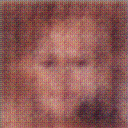
\includegraphics[width=150px]{500_fake_images/samples_5_430.png}%
\caption{A Man With A Beard Wearing A Tie}%
\end{figure}

%
\end{document}